\documentclass[a4paper,11pt]{report}
\usepackage[T1]{fontenc}
\usepackage[utf8]{inputenc}
\usepackage[italian]{babel}
\usepackage{lmodern}
\usepackage{hyperref}
\usepackage{graphicx}
\usepackage{wrapfig}
\usepackage{listings}

\selectlanguage{italian}
\title{TITOLO PROVVISORIO}
\author{Matteo Martelli}

\begin{document}

\maketitle
\tableofcontents

\begin{abstract}
\end{abstract}

\chapter{Introduzione}

\section{Scenari di Disaster Recovery}

\section{STEMNET}

\section{Oltre la simulazione}

\chapter{Piano di Processo}

\section{Motivazioni}

\section{Obbiettivi}
Gli obbiettivi sono..

\section{Scenario di STEMNET}

\section{Scenario di Progetto}
\begin{figure}
\centering
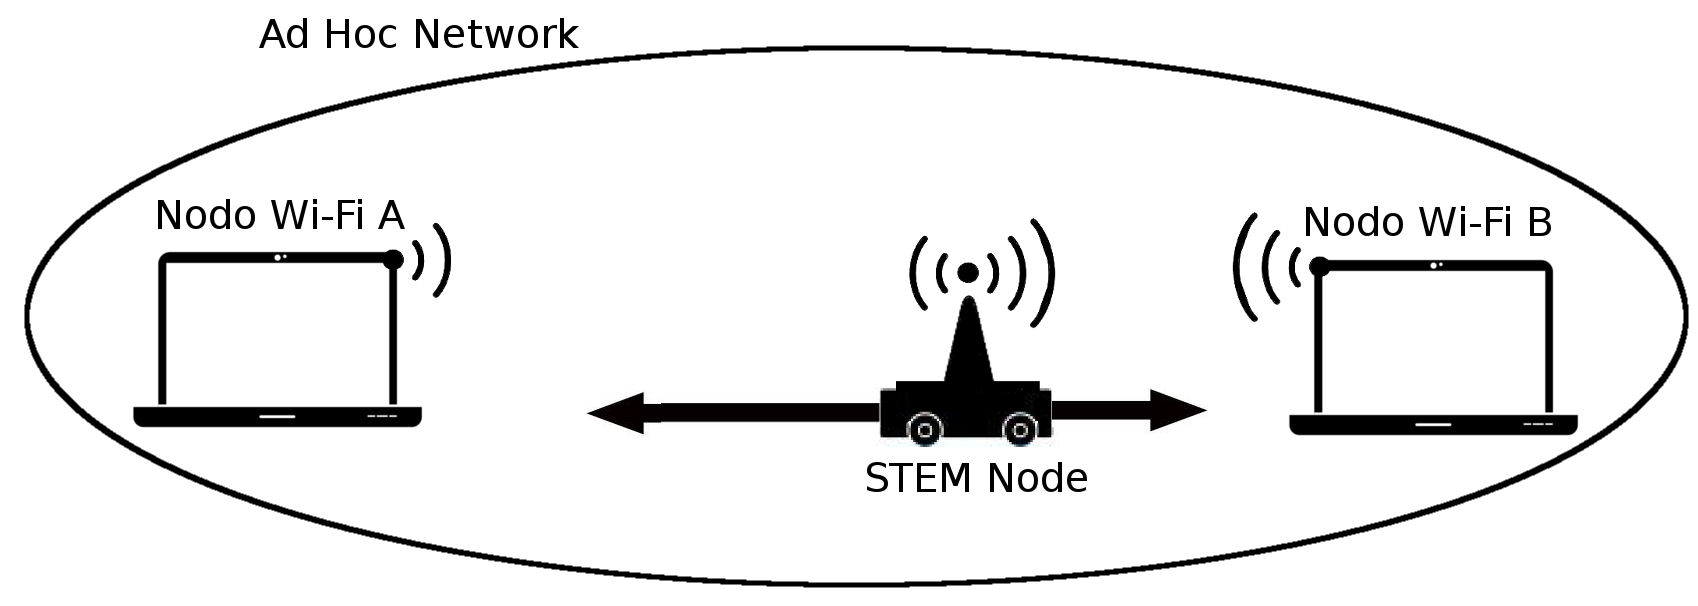
\includegraphics[scale=0.25]{scenario.png}
\caption{Schema dello scenario di progetto}
\end{figure}
Nel progetto si fa riferimento ad uno scenario semplificato rispetto a quello esposto in STEMNET.
Ci si vuole ridurre al caso di un singolo sensore STEM-Node (SN) in modo da poterne studiare nello specifico le possibilità implementative.
L'idea è quella di posizionare l'SN tra altri due nodi Wi-Fi simulatori, i quali simulerebbero appunto il comportamento delle isole o, tramite movimento manuale l'azione di altri SN. 
Il sistema di tutti i nodi Wi-Fi (SN compreso) viene distribuito su una linea retta per facilitarne lo studio iniziale, eliminando le problematiche della determinazione della posizione geografica dei nodi (ci si focalizza sul movimento dipendente esclusivamente dal Link Budget).
Una volta che lo sviluppo di un singolo SN sarà terminato e testato, si passerà ad ampliare lo scenario aggiungendo molteplici SN, apportando le opportune modifiche hardware e software, studiandone poi il comportamento.



\section{Analisi dei Requisiti}
Lo scenario di progetto richiede che:
\begin{itemize}
\item
l'SN sia dotato di almeno un modulo radio (Wi-Fi in questo caso), tramite il quale l'SN possa percepire la potenza di segnale di altri punti radio nel suo raggio di ricezione (determinato dalla sensibilità dello stesso modulo).
\item
l'SN si possa muovere autonomamente e che quindi possa controllare uno o più dispositivi di movimento, quali uno o più motori con delle ruote o delle eliche se si pensa ad un contesto aereo.
\item
l'SN sia in grado di ricevere e trasmettere del traffico di rete, permettendo quindi la comunicazione tra i due nodi Wi-Fi estremi al sistema, anche qual'ora essi non siano nello stesso raggio di copertura.    
\end{itemize}

\section{Risorse e strumenti impiegati}
\begin{itemize}
  \item Hardware
  \begin {itemize}
    \item Arduino Uno: piattaforma hardware programmabile tramite seriale USB. 
      Monta un microcontrollore ATmega328P, 14 pin I/O digitali e 6 pin I/O analogici.\\
      \url{http://arduino.cc/en/Main/ArduinoBoardUno} 
    \item Magician Chassis ROB-10825: piattaforma robot. Monta due motori con ruote da 65mm e una rotella posteriore.\\
        \url{https://www.sparkfun.com/products/10825}
    \item Motor Driver 1A Dual TB6612FNG: scheda per il controllo dei motori. Può controllare fino a due motori.\\
        \url{https://www.sparkfun.com/products/9457}
    \item Wireless Proto Shield: scheda per connettere facilmente dei moduli wireless all'Arduino board.\\
        \url{http://arduino.cc/en/Main/ArduinoWirelessProtoShield}
    \item WiFly Shield RN-XV: scheda che incorpora il modulo Wi-Fi RN171. Permette di connettersi ad una rete Wi-Fi 
        in modalità infrastructure o Ad-Hoc.\\
        \url{http://rovingnetworks.com/products/RN171XV}
    \item Due interfaccie Wi-Fi su sistema GNU Linux.  
  \end {itemize}
  \item Software e Linguaggi di Programmazione
  \begin {itemize}
    \item Wiring per Arduino: è una piattaforma di sviluppo open source composta da un linguaggio di programmazione derivato da C e C++ ed un ambiente di sviluppo integrato (Integrated Development Environment o IDE) con elementi per gestire l'hardware dell'Arduino Board.
    \item Python per la parte di applicazione GNU Linux.
  \end{itemize}
  
\end{itemize}


\chapter{Progettazione}
\begin{wrapfigure}{l}{0.3\textwidth}
  %\begin{center}
    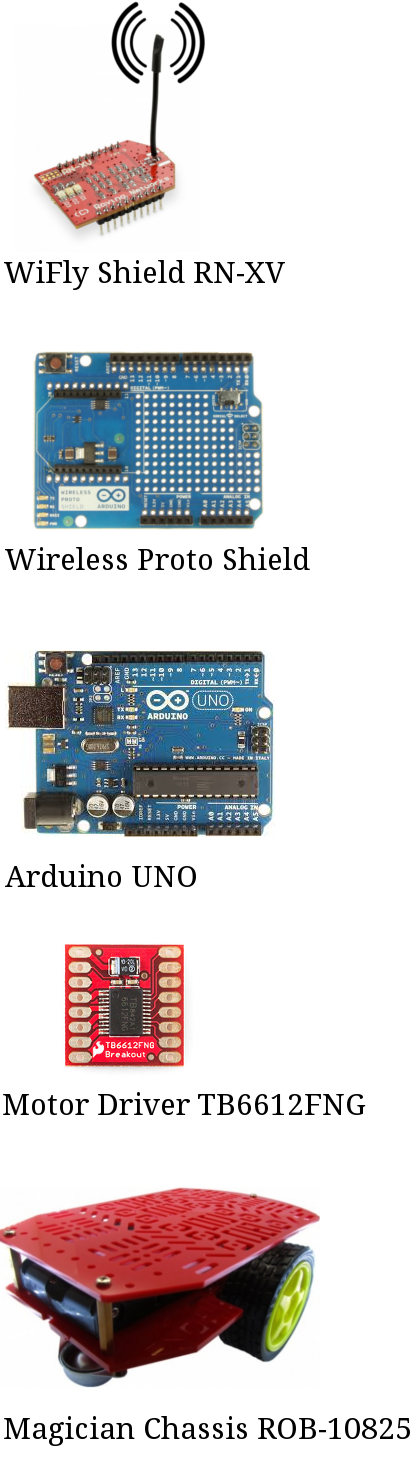
\includegraphics[scale=0.25]{sn.png}
  %\end{center}
\end{wrapfigure}
Si è scelto di utilizzare i componenti hardware elencati nella sezione "Risorse e strumenti impiegati" affinchè potessero venir soddisfatti i requisiti specificati in "Analisi dei Requisiti".\\ 
L'SN consiste quindi di un Arduino UNO collegato ad un'unità mobile (Magician Chassis ROB-10825) composta da due motori utilizzati per il movimento ed ad un modulo Wi-Fi(WiFly Shield RN-XV).\\
I motori vengono controllati tramite un motor driver (Motor Driver 1A Dual TB6612FNG) al quale il microcontrollore trasmette in output tensione modulata in tipo PWM dai pin digitali. In questo modo si riesce a comunicare ai motori anche una certa velocità. \\
Il modulo Wi-Fi è collegato all'Arduino tramite una Wireless Shield che non fa altro che interfacciare il modulo Wi-Fi all'Arduino tramite una connesione seriale attraverso la quale le due schede comunicano.\\

Si è scelto di lavorare con una rete in modalità ad-hoc affinchè in una futura estensione dell'implementazione, tutti gli SN possano conoscere la potenza di segnale ricevuta (RSSI) dai nodi della rete all'interno loro raggio di copertura. %Questo è possibile in una rete ad-hoc in quanto ogni nodo manda dei pacchetti beacon periodici con all'interno, tra le altre informazioni sulla rete, l'RSSI...%TODO verificare come 
Nel nostro caso il firmware del modulo Wi-Fi scelto non supporta alcuna funzione per ottenere gli RSSI di più nodi all'interno di una rete Ad-Hoc, quindi per il momento gli RSSI vengono inviati direttamente dai due nodi Wi-Fi tra cui l'SN è posizionato (come già specificato nello scenario di progetto). Questo viene fatto da un programma che gira su entrambi i nodi Wi-Fi simulatori. Il programma invia pacchetti UDP periodici all'SN con all'interno del payload la potenza di segnale ricevuta da esso.\\
Per questa parte della progettazione, la soluzione appena descritta è sufficiente per permettere lo studio del movimento dell'SN e delle sue reazioni in base alle dinamiche del sistema. Successivamente verranno descritte delle soluzioni alternative possibili per lo sviluppo di una futura implementazione.          

%TODO spiegazione algoritmo stemnet
La parte software è divisa essenzialmente nelle due parti spiegate di seguito.
\section{Programma Python per sistemi GNU Linux}
  Il programma scritto in python per sistemi GNU Linux, come descritto precedentemente, semplicemente invia periodicamente dei pacchetti UDP all'SN con all'interno l'RSSI ricevuto dall'SN. Per ottenere l'RSSI, il programma utilizza l'utility iw \url{http://wireless.kernel.org/en/users/Documentation/iw}. Questa utility permette di elencare, divisi per MAC address, tutti i nodi presenti nella rete Ad-Hoc, con le relative potenze di segnale. Quindi essendo a conoscenza del MAC address dell'SN, ogni nodo Wi-Fi simulatore, può determinare il proprio RSSI correlato all'SN ed inviarglielo. 
\section{Programma Wiring per Arduino}
  Il programma scritto in Wiring per Arduino è la parte di software cuore del progetto. Come già accennato in precedenza, "Wiring" generalmente è una piattaforma di sviluppo open source composta da un linguaggio di programmazione, un ambiente di sviluppo integrato (Integrated Development Environment o IDE) ed un circuito stampato basato su un microcontrollore. Nel nostro caso il linguaggio di programmazione è composto da un ibrido tra C e C++ creato appositamente dal team Arduino. Lo stesso team ha messo a disposizione anche un IDE apposito che facilita l'interfacciamento alla board Arduino (scrittura del codice, compilazione e flashing). Tramite questa parte l'Arduino riesce a controllare il suo movimento, analizzando la potenza di segnale dei nodi connessi alla rete stabilendo se muoversi, in quale direzione e con quale velocità. Prima di effettuare la decisione l'Arduino analizza se la rete è critica ovvero se è a rischio di rottura. Inoltre a priori viene stabilito un fattore di attenuazione della forza di movimento che, insieme alla criticità della rete, costituiscono una "Probabilità di Movimento". L'SN quindi tiene in considerazione la probabilità di movimento prima di prendere la decisione. Questo comporta che l'SN non si muoverà se il rischio di rottura della rete è alto e diminuirà la sua reazione a piccoli stimoli con l'aumentare del fattore di attenuazione. I dettagli implementativi verranno spiegati di seguito nel capitolo 4.

\chapter{Implementazione}
\section{Implementazione del client UDP Python}
Come già accennato in precedenza, si è scelto di realizzare un programma python per ovviare al problema dell'assenza di un modo che consenta al modulo Wi-Fi utilizzato di ottenere l'RSSI dei nodi nella rete Ad-Hoc. L'idea è quella di utilizzare l'utility iw per i sistemi operativi GNU Linux. L'utility iw è basata su nl80211, l'interfaccia utente in fase di sviluppo per netlink, una famiglia di socket utilizzata per IPC (Inter-process communication) tra il kernel e i processi in user-space.\\
Per ottenere le informazioni dei nodi connessi alla stessa rete ad hoc della macchina in questione, basta il comando:
\begin{lstlisting}
$ iw dev <devname> station dump
\end{lstlisting}
dove <devname> è il nome dell'interfaccia Wi-Fi che si vuole utilizzare.
In output fornisce le informazioni nel formato seguente:

%TODO

Se si vogliono avere le informazioni specifiche di un solo nodo è invece sufficiente il seguente comando:
\begin{lstlisting}
$ iw dev <devname> station get <peer-MAC-address>
\end{lstlisting}
dove <peer-MAC-address> identifica l'indirizzo MAC dello specifico nodo.
Nel caso in cui l'interfaccia sia connessa ad una rete in modalità infrastructure, l'output del comando restituirà solo le informazioni degli AP che costuiscono la rete, ma non dei client.\\
C'è da specificare che il tutto è possibile solo se i driver dell'interfaccia Wi-Fi utilizzata supportano nl80211. \\
Adesso il programma non fa altro che inviare ogni $n$ secondi fissati, un pacchetto UDP con il payload composto in questo modo:
\begin{lstlisting}
###IP_ADDRESS,MAC_ADDRESS,RSSI;
\end{lstlisting}
ed ad esempio:
\begin{lstlisting}
###10.42.1.11,00066671e1b7,-31;
\end{lstlisting}
Il formato scelto non ha una particolare importanza, stabilisce solo una convenzione nota tra i client e l'SN che dovrà scansionare e fare il parsing del pacchetto ricevuto.  
\end{document}
